% !TeX spellcheck = en_GB

% List of packages and options for them
% Base packages
\documentclass[a4paper,10pt]{article}
\usepackage{a4wide} \bibliographystyle{plain}
\usepackage[english]{babel}
\usepackage{parskip} % To prevent indentation of new paragraphs
\usepackage[utf8]{luainputenc}
%\usepackage{bibentry} \usepackage{cite} \bibliographystyle{plain} % For bibliographies
\usepackage{placeins} % Barrier for floats
%\usepackage{pdfpages} % Include pdfs in your document
%\usepackage{eurosym} % Include the euro symbol

% Text layout packages
\usepackage[hidelinks]{hyperref}
\usepackage{color} % For fancy colors
\usepackage{enumitem} % For lists
%\usepackage{multicol} % For multi-column texts
\usepackage{fontspec} % For custom fonts
%\usepackage{titling} % For custom size titles
%\usepackage{soul} % For strikethrough text

% Figures & References packages
\usepackage[labelfont=bf]{caption} \captionsetup{width=0.8\textwidth, font=small} % For captions
\usepackage{subcaption} % For more advanced captions, such as figure 1a, b, c
%\usepackage{wrapfig} % For figures on the side of the text
%\usepackage{epstopdf} % To be able to include eps files
%\usepackage{graphicx} % Include more types of images

% Graphs packages
\usepackage{tikz} % Used for custom vectors and other drawings
%\usetikzlibrary{decorations.pathmorphing,patterns,arrows,arrows.meta,calc,angles,quotes} % Tikz packages for drawing figures
%\usetikzlibrary{external} \tikzexternalize[prefix=graphs/] % Cached tikz graphics
%\usepackage{pgfplots} \usepgfplotslibrary{fillbetween,patchplots} \pgfplotsset{compat=newest} % For fancy graphs
%\usepackage{pgfplotstable} % To use tables as data source for graphs
%\usepackage{filecontents} % To export content to a given file from latex

% Table packages
%\usepackage{booktabs} % Used for lines in tables
%\usepackage{array} % For vertical alignment of text in cells
%\usepackage{longtable} % For page-spanning tables
%\usepackage{multirow} % For row-spans besides column-spans

% Computing Science packages
\usepackage{listings} % For code listings
\usepackage{minted} % For code coloring (requires color)

% Maths packages
%\usepackage{amsmath} % For most maths things
%\usepackage{physics} % For derivative sign things
%\usepackage{mathtools} % More maths things (fixes things in amsmath, requires it as well)
%\usepackage{amssymb} % Special symbols
%\usepackage{gensymb} % Degree symbol
%\usepackage{mathdots} % Special dots

% Physics packages
%\usepackage{siunitx} \sisetup{load-configurations = abbreviations, separate-uncertainty=true, exponent-product=\cdot, output-product=\cdot} % Si units!
%\usepackage{mhchem} % Chemical equations package

% Code style definitions
\definecolor{Gray}{gray}{0.95}

\setsansfont{Segoe UI}
\newfontfamily{\consolas}{Consolas}
\renewcommand{\theFancyVerbLine}{\sffamily\textcolor[rgb]{0.5,0.5,0.5}{\scriptsize\arabic{FancyVerbLine}}}
\usemintedstyle{vs}
\usemintedstyle[Matlab]{lovelace}

\newminted[matlong]{Matlab}{
	linenos,
	frame=lines,
	framesep=3mm,
	breaklines,
	breakautoindent=true,
	fontsize = \fontsize{8pt}{10.5pt},
%	fontsize = \footnotesize,
	tabsize = 4,
	bgcolor=white
}

\newminted[mats]{Matlab}{
	tabsize = 4,
	breaklines,
	breakautoindent=true,
	bgcolor=white
}

\newmintinline[mat]{Matlab}{
	mathescape,
	tabsize = 4
}

\overfullrule=1cm
\showboxdepth=\maxdimen
\showboxbreadth=\maxdimen

\title{A no-nonsense beginner's tool for GMLVQ}
\author{Version 3.0}

% Leaders
\newcommand*{\titlerule}[3][]{%
  \makebox[#2]{#1%
    \leaders\hrule height \dimexpr.5ex+.2pt\relax depth \dimexpr -.5ex+.2pt\relax \hfill% Left rule
    \enskip{#3}\enskip% Text (and surrounding spaces)
    \leaders\hrule height \dimexpr.5ex+.2pt\relax depth \dimexpr -.5ex+.2pt\relax \hfill\kern0pt}% Right rule
	\vspace{3pt}
}

% Middle of text comment
\newcommand{\comment}[2]{%
	\vspace{6pt}
	\makebox[\linewidth][c]{%
		\begin{minipage}{.9\linewidth}
			\titlerule{\linewidth}{\footnotesize\bf#1}
			#2
			\vspace{8pt}\hrule
		\end{minipage}
	}
	\vspace{6pt}
}

% Better vectors in latex
\makeatletter
\newlength\xvec@height%
\newlength\xvec@depth%
\newlength\xvec@width%
\newcommand{\xvec}[2][]{%
	\ifmmode%
	\settoheight{\xvec@height}{$#2$}%
	\settodepth{\xvec@depth}{$#2$}%
	\settowidth{\xvec@width}{$#2$}%
	\else%
	\settoheight{\xvec@height}{#2}%
	\settodepth{\xvec@depth}{#2}%
	\settowidth{\xvec@width}{#2}%
	\fi%
	\def\xvec@arg{#1}%
	\def\xvec@dd{:}%
	\def\xvec@d{.}%
	\raisebox{.2ex}{\raisebox{\xvec@height}{\rlap{%
		\kern.05em%  (Because left edge of drawing is at .05em)
		\tikzset{external/export=false}%
		\begin{tikzpicture}[scale=1]
		\pgfsetroundcap
		\draw (.05em,0)--(\xvec@width-.05em,0);
		\draw (\xvec@width-.05em,0)--(\xvec@width-.15em, .075em);
		\draw (\xvec@width-.05em,0)--(\xvec@width-.15em,-.075em);
		\ifx\xvec@arg\xvec@d%
		\fill(\xvec@width*.45,.5ex) circle (.5pt);%
		\else\ifx\xvec@arg\xvec@dd%
		\fill(\xvec@width*.30,.5ex) circle (.5pt);%
		\fill(\xvec@width*.65,.5ex) circle (.5pt);%
		\fi\fi%
		\end{tikzpicture}%
	}}}%
	#2%
}
\makeatother

% --- Override \vec with an invocation of \xvec.
\let\stdvec\vec
\renewcommand{\vec}[1]{\xvec[]{#1}}
% --- Define \dvec and \ddvec for dotted and double-dotted vectors.
\newcommand{\dvec}[1]{\xvec[.]{#1}}
\newcommand{\ddvec}[1]{\xvec[:]{#1}}
\newcommand{\iu}{{i\mkern1mu}}

% Some sizing hack
\newsavebox{\measuredSize}
\newcommand{\resizeToWidth}[2]{%
	\pgfmathsetmacro{\pgfplotswidth}{#2}%
	\begin{lrbox}{\measuredSize}#1\end{lrbox}%
	\pgfmathsetmacro{\pgfplotswidth}{2*\pgfplotswidth-\wd\measuredSize}%
	#1%
}

\begin{document}
\maketitle

\vspace{350pt}
\comment{Disclaimer}{
This demonstration software, referred to as `GMLVQ demo code', or `A no-nonsense beginner's tool for GMLVQ', is provided `as is' and any expressed or implied warranties are disclaimed.

In no event shall the author or any contributors be liable for any direct, indirect, incidental, special, exemplary, or consequential damages. This demonstration software should not be used for critical applications.
}

\newpage

\section{Getting started}
To get started using this library in Matlab, you'll need to first set up the library correctly. This can be done by extracting the archive into some directory, and adding that directory to your Matlab path. Alternatively, start Matlab in that directory directly. You can test whether the library loaded correctly by trying to type the first letters of `GMLVQ' in the console and trying the autocomplete by hitting {\tt [Tab]}. It should automatically complete the name.

Secondly, you'll need a properly formatted and labelled data set. Specifically, you'll need two variables {\tt fvec} and {\tt lbl}. {\tt fvec} should be an array of size {\tt nFv x nDim}, containing the set of {\tt nFv} feature vectors in {\tt nDim} dimensions. {\tt lbl} should be a corresponding vector of {\tt nFv} class labels. These labels must cover the complete set 1-{\tt nFv}. As an example, a number of sample data sets are provided in the archive, those will also be used in the demonstrations later on.

All functionality of the library is put inside of the {\tt GMLVQ}-namespace. There are a number of classes, each class with a number of functions, to assist you in using the library intuitively. This means that each classname should be prepended with {\tt GMLVQ.} in the code.

\section{Examples}
Most functionality of the library will be covered in the following examples, they should give you an idea of how the library should be used and what results you can obtain with it. For more detailed information on the API, later on there will be a complete reference.

\subsection{Initialization}
To be able to run the algorithm, you will first need to obtain an instance of the {\tt GMLVQ.GMLVQ}-class. This class stores your data set, as well as the parameters you have chosen for the algorithm. Using this class, it is possible to run various tests on the data set and obtain results. This class can be instantiated using the following constructor:

\begin{mats}
GMLVQ.GMLVQ(fvec, lbl, parameters, totalsteps, prototypeLabels)
\end{mats}
%
Here, {\tt fvec} and {\tt lbl} are the variables discussed above. {\tt parameters} must be an instance of {\tt GMLVQ.Parameters}, where you can set various parameters for the algorithm. {\tt totalsteps} is the number of time steps to take while running the algorithm (by default: 10), and lastly {\tt prototypeLabels} is a vector specifying how many prototypes, and for which classes to use. By default this is simply one prototype per class, but by setting this variable it is possible to use multiple prototypes per class.

As mentioned above, the {\tt GMLVQ.Parameters}-class contains all parameters to use in the algorithm. This class can be instantiated using a name-value style call of the constructor, for example as follows:

\begin{mats}
GMLVQ.Parameters('paramName', value, 'paramName2', value2, ...)
\end{mats}
%
The following parameters can be set in this class, including their type and default (recommended) values. More context on some of these options will be given in later examples.
\begin{itemize}
\item \mat!mode = GMLVQ.Mode.GMLVQNS! ({\tt GMLVQ.Mode} enum): The mode to use for the algorithm. Put in one of the elements from the enum {\tt GMLVQ.Mode}:
	\begin{itemize}
	\item {\tt GMLVQ.Mode.GMLVQ}: Matrix without null-space correction
	\item {\tt GMLVQ.Mode.GMLVQNS}: Matrix with null-space correction
	\item {\tt GMLVQ.Mode.GRLVQ}: Diagonal matrix (discouraged)
	\item {\tt GMLVQ.Mode.GLVQ}: GLVQ with Euclidian distance
	\end{itemize}
\item \mat!doztr = true! (boolean): Whether or not to do a z-score transformation on the training data.
\item \mat!rndinit = false! (boolean): When {\tt true}, will randomize the initialization of the relevance matrix, instead of using the identity matrix. {\tt false} is recommended for first experiments.
\item \mat!mu = 0! (real): A control parameter of the penalty term when lambda is singular. A value of 0 means default GMLVQ behaviour and is recommended for first experiments. Values larger than 0 prevent a singular lambda matrix, while values much larger than 0 let lambda approach identity, i.e. Euclidian behaviour.
\item \mat!decfac = 1.5! (real): Step size factor (decrease) for Papari steps
\item \mat!incfac = 1.1! (real): Step size factor (increase) for all steps
\item \mat!ncop = 5! (integer): Number of waypoints stored and averaged during the algorithm calculation.
\item \mat!etam! (real): Stepsize adaptation parameter. Default value 2 for GMLVQ or GMLVQNS modes, 0.2 for GRLVQ and 0 for GLVQ.
\item \mat!etap! (real): Stepsize adaptation parameter. Default value 1 for GMLVQ or GMLVQNS modes, 0.1 for GRLVQ and 1 for GLVQ.
\item \mat!rngseed = 291024! (integer): The seed to use for the random number generator to allow for reproducible results.
\item \mat!rocClass = 1! (integer): The label of the class to compute the ROC against.
\item \mat!showlegend = true! (boolean): Whether or not to show legends in the graphs produced upon plotting.
\item \mat!randomization = 0.02! (real): A measure for how `spread out' the initial prototype locations are for execution. Will not affect results when {\tt useKMeans} is {\tt true}.
\item \mat!useKMeans = true! (boolean): Whether or not to use k-means to initialize the prototypes.
\end{itemize}

So combining this, if I want to run the algorithm without the k-means initialization, running for 50 steps, using two prototypes for the second class, I could call the following in the console:
\begin{mats}
gmlvq = GMLVQ.GMLVQ(fvec, lbl, GMLVQ.Parameters('useKMeans', false), 50, [1 2 2 3 4]);
\end{mats}

\subsection{Single runs of GMLVQ}
In this section we will only be using the \mat!runSingle()! function of the {\tt GMLVQ}-class. This function performs a single training process for the entire data set. The result is an instance of the {\tt Result}-class, which includes a bunch of performance statistics, such as the cost function, error rates and AUROC as functions of time(steps) and the final LVQ system.

Using the \mat!plot(...)! function you can plot the training curves, the final LVQ system is visualized in terms of prototype vectors and the relevance matrix, and the ROC of the final system is displayed. The data set is also visualized in terms of the leading two eigenvectors of the relevance matrix.

\newpage
\subsubsection{Demo I: A seven-class data set, single run with one prototype per class}
This is the UCI segmentation data set, where 1 trivial dimension was removed and 800 samples were randomly selected. From the results, it is clear that classes 2 and 7 are easily distinguishable, while classes 3 through 6 lie very close together. This can also be seen in the class-wise training errors. In the resulting figure, the ROC (w.r.t. class 1) is not shown.
\begin{matlong*}{label=\textrm{Console session}}
>> load uci-segmentation-sampled.mat
>> gmlvq = GMLVQ.GMLVQ(fvec, lbl, GMLVQ.Parameters(), 50);
Matrix relevances with null-space correction
Defaulted to one prototype per class
Prototype configuration:
     1     2     3     4     5     6     7
Warning: Multi-class problem. ROC analysis is for class 1 (neg.) vs. all others (pos.) 
Minimum standard deviation of features: 0.025258
>> result = gmlvq.runSingle();
>> result.plot();
\end{matlong*}
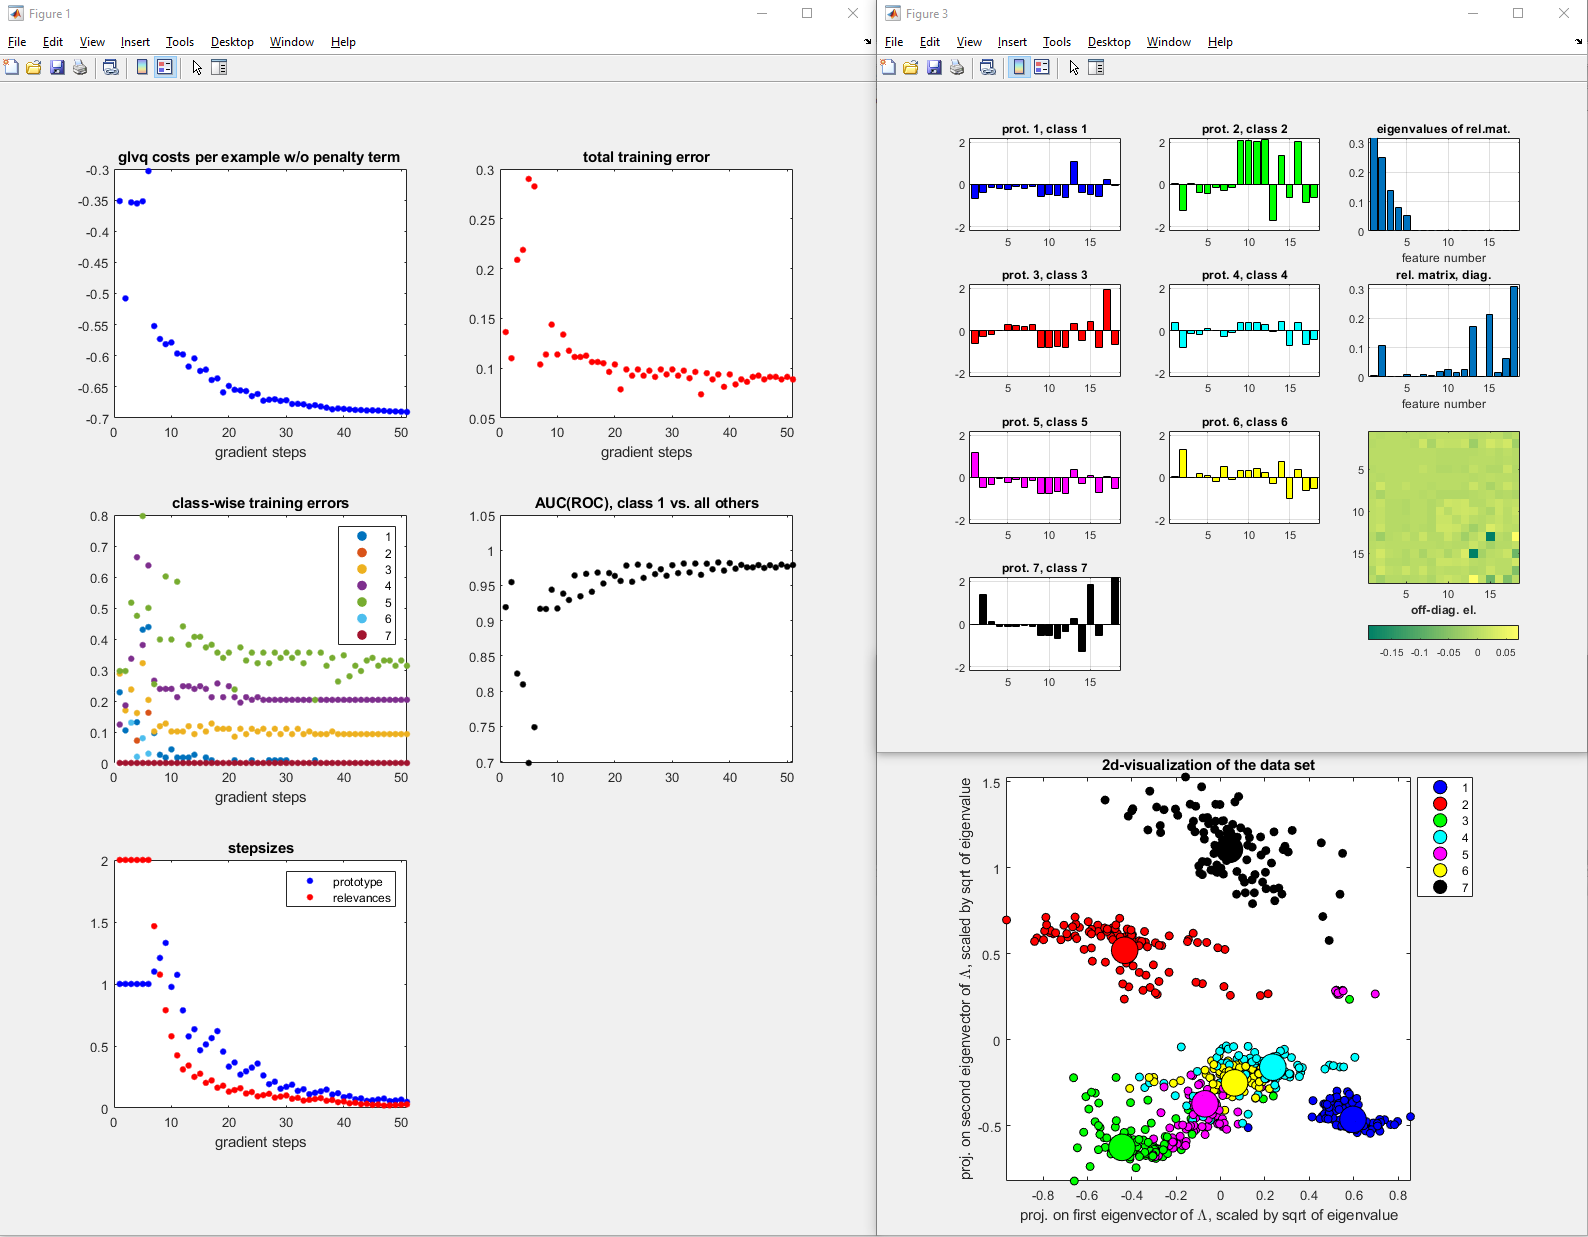
\includegraphics[width=\linewidth]{demos/demo1.png}

\newpage
\subsubsection{Demo II: A simple two-class problem, single run with one prototype per class, ROC against class 1}
This data set has 186 features for 110 samples, but yields a very clear separation between both its classes.
\begin{matlong*}{label=\textrm{Console session}}
>> load twoclass-simple.mat
>> gmlvq = GMLVQ.GMLVQ(fvec, lbl, GMLVQ.Parameters('rocClass', 1), 30);
Matrix relevances with null-space correction
Defaulted to one prototype per class
Prototype configuration:
     1     2
Minimum standard deviation of features: 0.0090926
>> result = gmlvq.runSingle();
>> plot(result); // Both calling styles work
\end{matlong*}
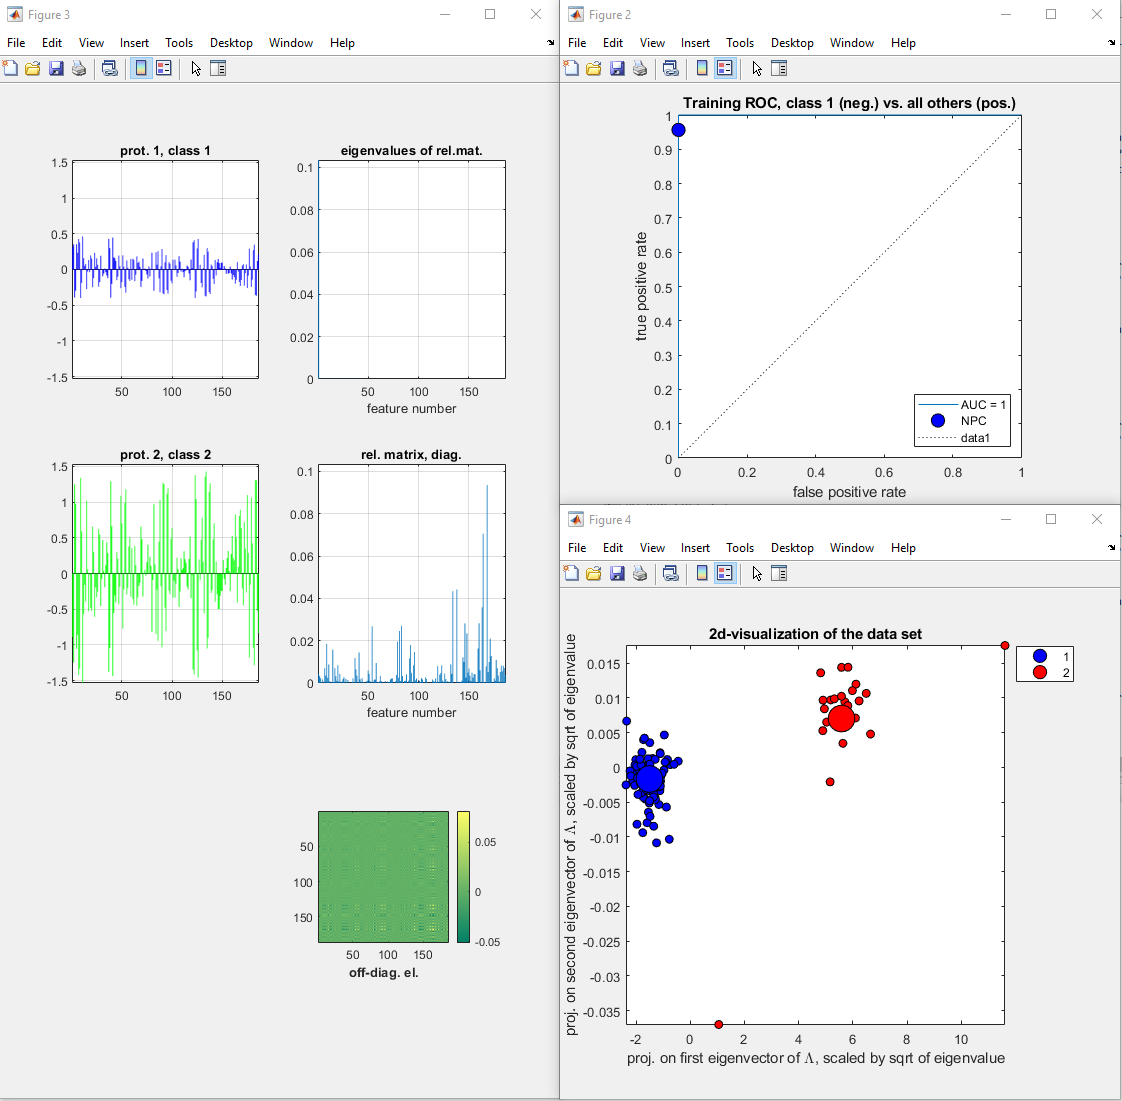
\includegraphics[width=\linewidth]{demos/demo2.png}

\newpage
\subsubsection{Demo III: A difficult two-class problem, single run with custom prototypes}
This data set has 32 features and 98 samples, but does not have a very clear separation.
\begin{matlong*}{label=\textrm{Console session}}
>> load twoclass-difficult.mat
>> gmlvq = GMLVQ.GMLVQ(fvec, lbl, GMLVQ.Parameters(), 50, [1 1 2]);
Matrix relevances with null-space correction
Prototype configuration:
     1     1     2
Minimum standard deviation of features: 0.56657
>> result = gmlvq.runSingle();
>> plot(result);
\end{matlong*}
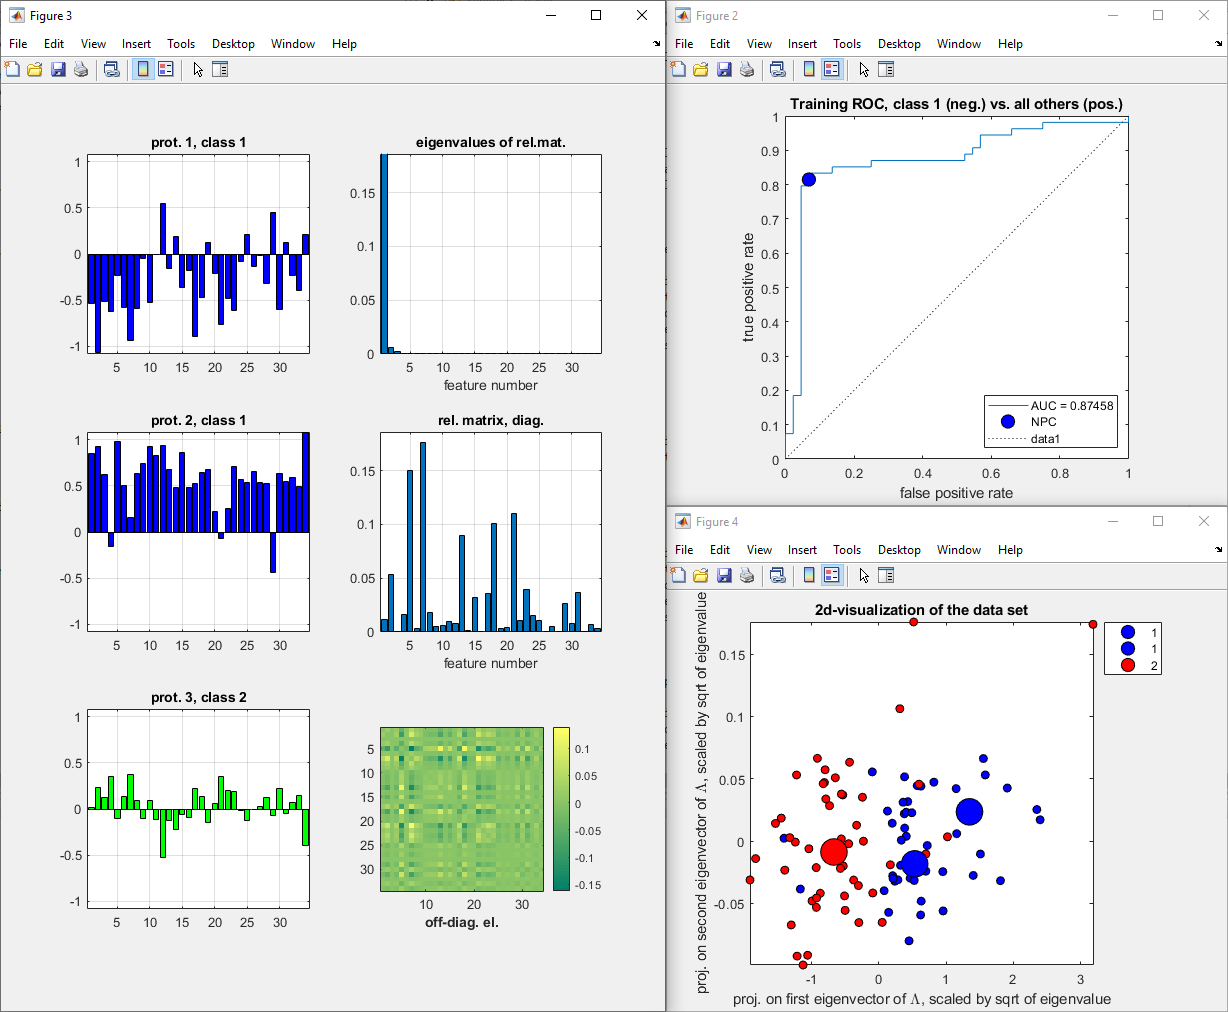
\includegraphics[width=\linewidth]{demos/demo3.png}
We can see that the eigenvalues are very close to singularity. To prevent this, we can tune the {\tt mu} parameter.
\begin{matlong*}{label=\textrm{Continued console session}}
>> gmlvq.params.mu = 0.2;
>> result = gmlvq.runSingle();
>> plot(result);
\end{matlong*}
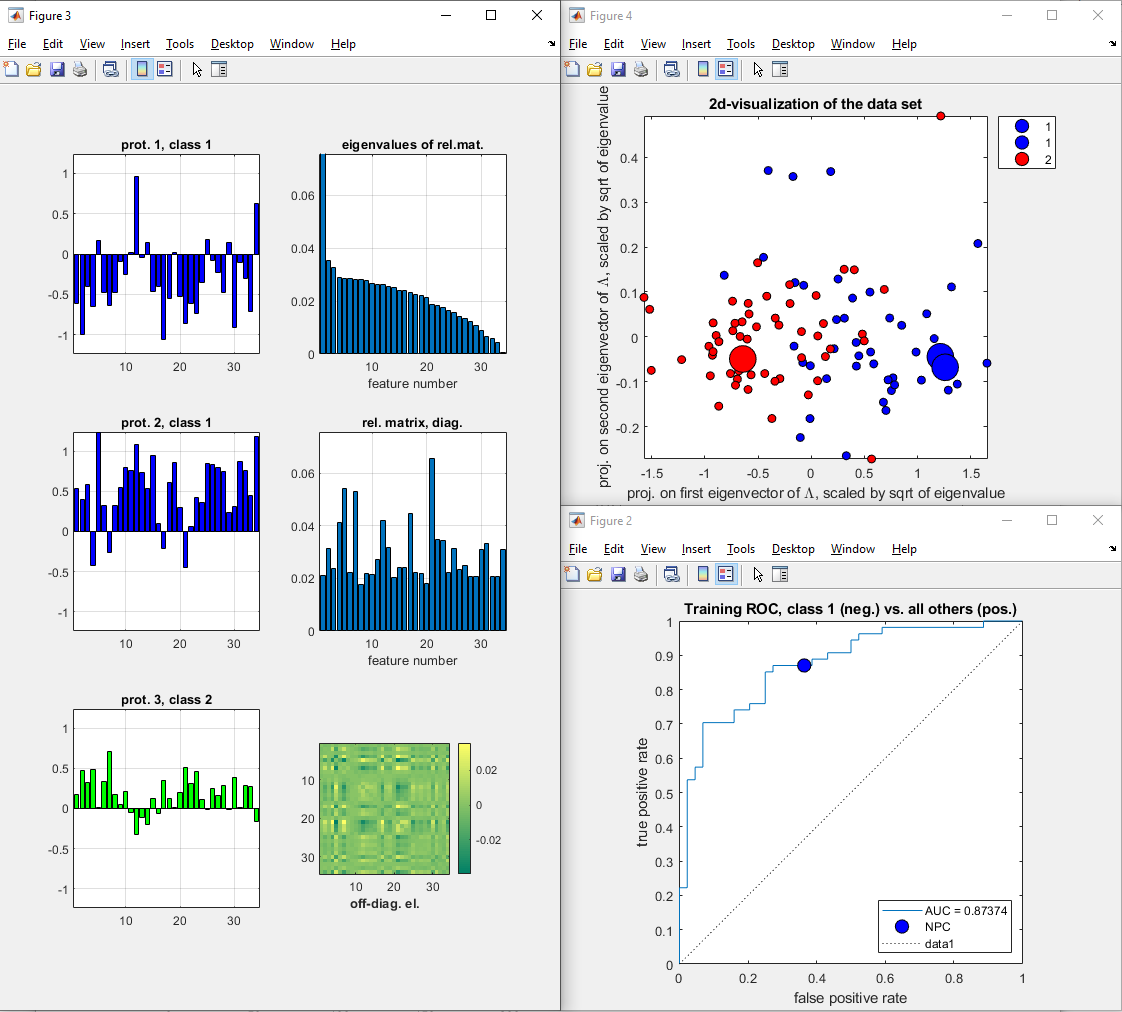
\includegraphics[width=\linewidth]{demos/demo4.png}

\newpage
\subsection{Multiple runs of GMLVQ}
In this section we will be discussion the \mat!runValidation(...)! and \mat!runL1O()! function of the {\tt GMLVQ}-class. These functions perform multiple training processes on a part of the data, while doing validation classification on the remaining data. They return an (specialized) instance of the {\tt ResultSet}-class, which includes the {\tt Result} instances for each run, as well as the average result where all properties are averaged. Again, using the \mat!plot(...)! function you can plot the entire resultset, or one of the subresults.

The \mat!runValidation(nRuns, percentage)! function runs {\tt n} times with {\tt percentage} of the data left out for validation. For each run, it makes a stratified partition of the data, i.e. the relative frequencies of the various classes will be kept constant and it will not happen that one class is completely omitted in one of the runs. In other words: {\tt percentage} of the samples \emph{per class} is left out.

The \mat!runL1O()! function runs {\tt nSamples} times, each time leaving out one sample for validation. L1O can seriously mis-estimate performance, and should really only be used for very small data sets.

\comment{Performance}{Performing multiple runs (especially L1O) can be really slow. Both the \mat!runValidation(...)! and \mat!runL1O()! functions parallelize the execution by performing each separate run in parallel. This is only possible if you have the Parallel Toolbox installed and activated, otherwise it will default to serial behaviour. Note that this also causes the output of the function to be out-of-order.}

\newpage
\subsubsection{Demo IV: A seven-class data set, multiple runs with 10\% of data left out}
This is the same data as in Demo I, so we have 800 samples. We see that the output of \mat!runValidation(...)! does not show ordered properly, this is because the code is run in parallel. Even when run in serial, it might show up out-of-order due to underlying code differences.
\begin{matlong*}{label=\textrm{Console session}}
>> load uci-segmentation-sampled.mat
>> gmlvq = GMLVQ.GMLVQ(fvec, lbl, GMLVQ.Parameters(), 40);
Matrix relevances with null-space correction
Defaulted to one prototype per class
Prototype configuration:
     1     2     3     4     5     6     7
Warning: Multi-class problem. ROC analysis is for class 1 (neg.) vs. all others (pos.)
Minimum standard deviation of features: 0.025258

>> result = gmlvq.runValidation(10, 10);
Learning curves, averages over 10 validation runs with 10% of examples per class left out for testing
Validation run 2 of 10
Validation run 4 of 10
Validation run 3 of 10
Validation run 6 of 10
Validation run 5 of 10
Validation run 1 of 10
Validation run 8 of 10
Validation run 9 of 10
Validation run 7 of 10
Validation run 10 of 10
>> plot(result);
\end{matlong*}
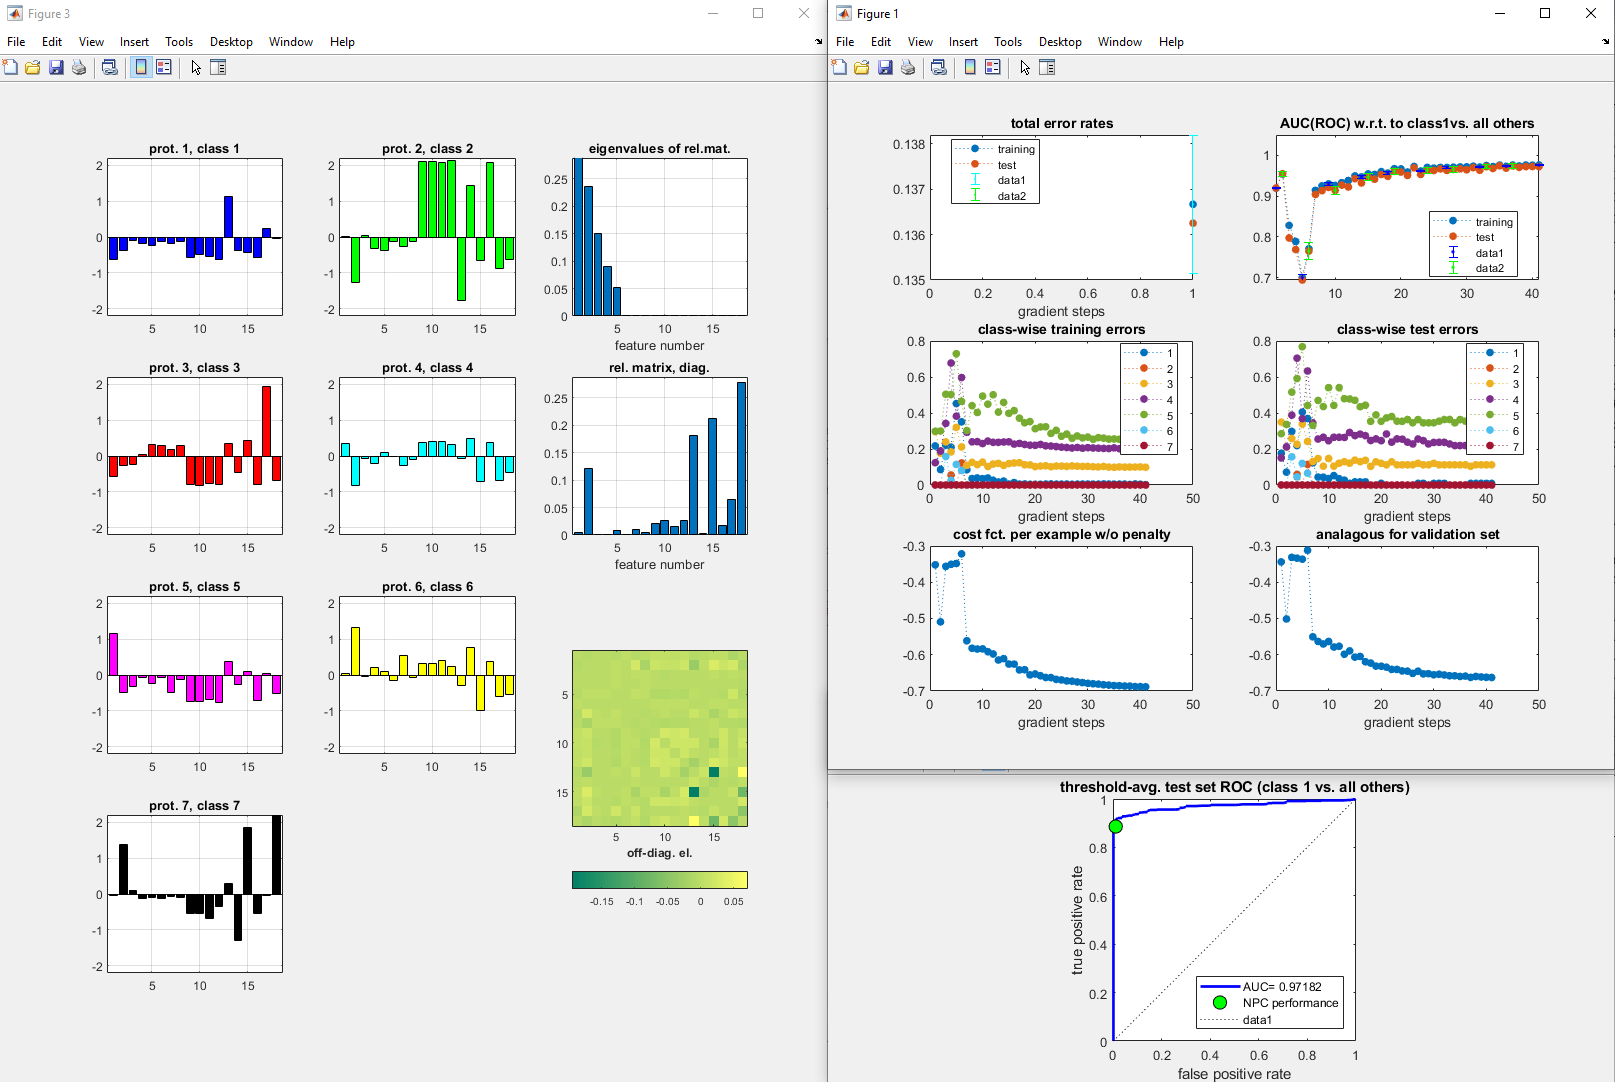
\includegraphics[width=\linewidth]{demos/demo5.png}

\newpage
\subsubsection{Demo V: A difficult two-class problem, validation with 10\% left out}
This is the same data as in Demo III, where the classification was not excellent. We will now run this 10 times with each time 10\% of the data left out. The code is similar to that of Demo IV.
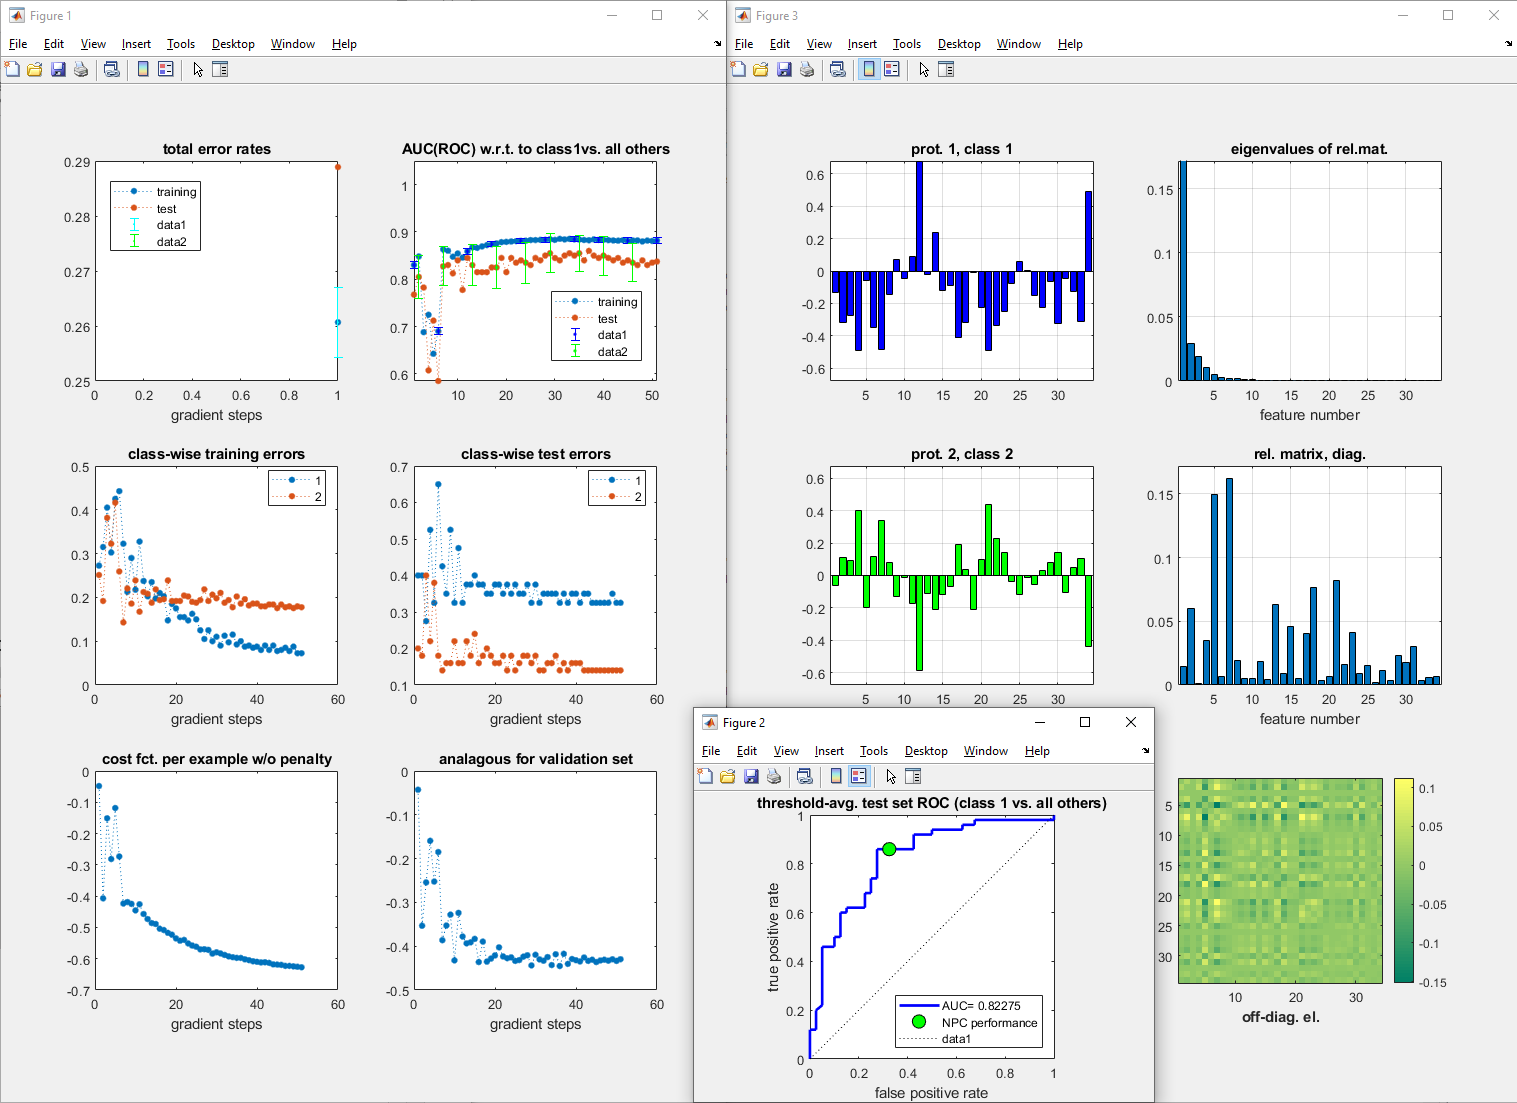
\includegraphics[width=\linewidth]{demos/demo6.png}
We can see that the validation performance is bad compared to the training performance (which we saw in Demo III), which hints at overfitting the data.

\newpage
\subsubsection{Demo VI: A small subset of a simple two-class problem, Leave-1-Out run}
In this case we only have a small subset of the data from Demo II, only 36 samples for 186 features. The best we can do here is to run L1O as last resort.
\begin{matlong*}{label=\textrm{Console session}}
>> load twoclass-simple-small.mat;
>> gmlvq = GMLVQ.GMLVQ(fvec, lbl, GMLVQ.Parameters(), 30);
Matrix relevances with null-space correction
Defaulted to one prototype per class
Prototype configuration:
     1     2
Minimum standard deviation of features: 0.0089232

>> result = gmlvq.runL1O();
Learning curves, averages over 36 L1O runs
Leave one out: 1 of 36
Leave one out: 8 of 36
....
Leave one out: 28 of 36
Leave one out: 35 of 36
>> plot(result);
\end{matlong*}
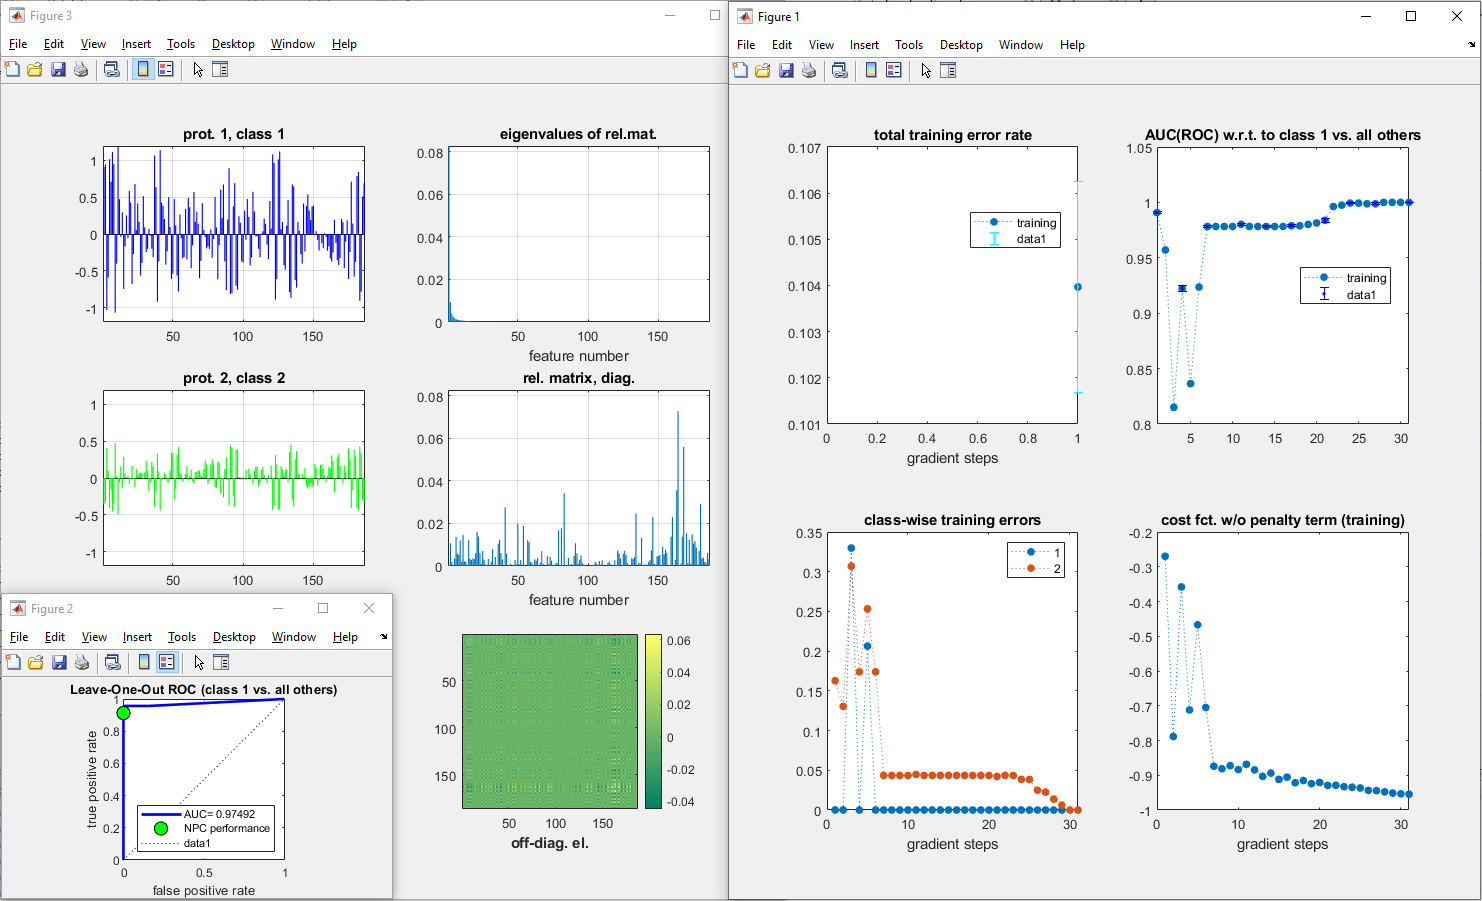
\includegraphics[width=\linewidth]{demos/demo7.png}

\newpage
\section{Changelog}
\subsection*{Main changes of version 3.0 (March 2019)}
\begin{itemize}[label=-]
\item Major API overhaul into an object-oriented design, allowing for re-use of parameters/run setups easily.
\item Possibility to store results to (re-)plot them later.
\item Parallelized the validation- and L1O-runs if the Parallel Toolbox is present.
\item Added possibility to calculate ROC vs. any class instead of just the class with label `1'.
\item Using {\tt cvpartition} in Matlab to obtain stratified training data for validation runs.
\item Added k-means prototype initialization instead of the previously used average of all points in the class.
\item Added a configurable option for the `randomness' of the initial prototypes (when not using k-means).
\item General performance improvements and code quality improvements
\end{itemize}

\subsection*{Main changes of version 2.3 (January 2017)}
\begin{itemize}[label=-]
\item Bug fixed in the averaging of prototypes over validation runs. Previous version yielded averaged prototypes that were stretched by a factor of 2, approximately. The error did not affect the training or validation itself, only the averaged prototypes in the final output.
\end{itemize}

\subsection*{Main changes of version 2.2 (April 2016)}
\begin{itemize}[label=-]
\item ROC calculation has been modified, it is now based on differences $d(x, w_1) - d(x, w_2)$ without normalization by $d(x, w_1) + d(x, w-2)$. See {\tt compute\_roc.m} for comments and details.
\end{itemize}

\subsection*{Main changes of version 2.1 (August 2015)}
\begin{itemize}[label=-]
\item Corrected legends in plots showing step size vs learning time
\item Corrected calculation of mean confusion matrix in \mat!run_validation(...)!. Now the confusion matrix is determined in each validation run separately (in terms of percentages) and then averaged over validation runs in the end. Resulting matrix is now in line with the averaged class-wise errors.
\end{itemize}

\subsection*{Main changes of version 2 (April 2015)}
\begin{itemize}[label=-]
\item Less explicit input parameters to functions (moved to function \mat!set_parameters(...)!)
\item Improved step size control, really independent for matrix and prototype updates
\item Singularity control via penalty term included, parameter {\tt mu} introduces
\item \mat!single_run(...)! also displays temporal evolution of step sizes
\item Null-space correction controlled in \mat!set_parameters(...)! (no dimension-dependent default anymore)
\item Initial step sizes independent of dimension and/or number of examples
\end{itemize}

\end{document}